\chapter[\paperIIItitle]{\texorpdfstring{%
                \paperIIItitle}{%
                \paperIIItitle}}

\label{ch:oscore}
\paperRemark{This is the full version of the paper below.
        This version contains an extended background description, and a more detailed motivation behind choices in the implementation as well as evaluation.
        \paperIIIref}
{i

\section{Introduction}
\label{s:introduction}

The Internet of Things (IoT) refers to a networked scenario where all connectable devices are reachable over the Internet and can communicate with each other. This has led to many new application scenarios, e.g. smart buildings, plant and home automation, smart electricity grids and smart transportation.

In such deployments, several IoT devices, also called \emph{nodes}, are units with limited resources such as memory, computing power and energy (if they are battery-powered). Having constrained resources results in constrained network segments, e.g. due to lossy channels and limited bandwidth \cite{rfc7228}. In order to cope with this, resource-constrained nodes tend to adopt an asynchronous and intermittent communication model, i.e. they handle network traffic according to sending/receiving timeslots. To save energy, nodes can go offline (\emph{sleep}), between two active timeslots, considerably extending their lifetime.

To manage these limitations, \emph{proxies} are used as intermediaries to enable access to server nodes that are not always online, by caching and forwarding requests.  With this in mind, the Constrained Application Protocol (CoAP) \cite{rfc7252} has been developed with support for proxying functionality, and is now a de-facto standard application-layer protocol for IoT. CoAP is a RESTful protocol, REST being an acronym for Representational State Transfer \cite{fielding2000architectural}. The REST model considers a Client and a Server as communicating parties, where the Client sends a Request to the Server, which replies by sending a Response. Based on the intended operation to perform, CoAP Requests can be of different types, e.g. GET, PUT, POST, FETCH, PATCH and DELETE.

Most applications require secure communications between client and server nodes. To this end, the CoAP specification \cite{rfc7252} considers Datagram Transport Layer Security (DTLS) \cite{rfc6347} as the only method to achieve secure communication for CoAP. In particular, DTLS establishes a secure channel at the \emph{transport layer} over unreliable datagram protocols such as UDP, and hence provides hop-by-hop security by protecting CoAP messages in their entirety. Due to proxies not being able to read encrypted CoAP messages, a DTLS channel must terminate at a proxy, so that the proxy can read the data needed for proxying functionality. As a consequence, a single DTLS channel cannot be established directly between the Client and the Server. Instead, a first secure channel has to be established between a Client node and the proxy, and then a second secure channel has to be established between the proxy and the Server node. This in turn results in the two following issues and limitations.

First, it is necessary to perform a double security processing of CoAP messages, as the proxy has to decrypt a message received on the client DTLS channel, and then re-encrypt the same message for delivery on the server DTLS channel, which impacts performance. Second, the proxy is necessarily required to be trusted, as it is able to fully access the CoAP messages. Mandating trust in proxies and the service providers operating them to such an extent results in unnecessary exposure of data.

This paper presents Object Security for Constrained RESTful Environments (OSCORE), an \emph{application-layer} approach for message protection based on \emph{object security} that efficiently overcomes these issues. To this end, OSCORE selectively protects certain parts of the CoAP messages at the application layer, providing \emph{end-to-end} secure communication between client and server nodes. In particular, some parts of CoAP messages can be encrypted, while other parts can be only authenticated and integrity-protected. This makes it possible to deploy non-trusted proxies, which are still able to perform their intended tasks. Furthermore, this greatly mitigates privacy threats otherwise possible for proxies to exploit, thus preserving the personal sphere of human users related to the information exchanged and the operations performed by the communicating endpoints. OSCORE has been recently standardized in the Internet Engineering Task Force (IETF) \cite{cite:oscoap}.

We have implemented OSCORE for the Contiki-NG OS \footnote{\url{https://github.com/contiki-ng/contiki-ng/wiki}}, and tested it on the resource-constrained platform Zolertia Firefly \footnote{\url{https://zolertia.io/product/firefly}} equipped with the CC2538 system-on-a-chip \footnote{\url{http://www.ti.com/lit/ds/symlink/cc2538.pdf}}. Then we used our implementation to experimentally evaluate OSCORE, considering a CoAP client and a resource-constrained CoAP server that securely communicate through a CoAP proxy.

In particular, we evaluated performance in terms of memory and CPU usage as well as energy consumption on the server side, and Round Trip Time experienced on the Client side. In our evaluation, we compared OSCORE performance against both an insecure baseline scenario using plain CoAP and a secure scenario using CoAP over DTLS. Our results show that OSCORE outperforms DTLS in terms of message overhead, round-trip time and energy efficiency, while still allowing a (non-trusted) proxy to perform its intended operations. To the best of our knowledge, this paper provides the first comprehensive performance evaluation of the standardized OSCORE protocol on a real IoT device, including a comparison against DTLS.

The rest of the paper is organized as follows. Section \ref{sec:related} presents the related work. Section \ref{sec:back} describes background technologies and concepts. Section \ref{sec:obj} provides the motivation behind this work, while Section \ref{sec:protocol} presents OSCORE. Section \ref{s:payloadoverhead} analyzes the overhead introduced by OSCORE, while Section \ref{sec:measure} describes our experimental setup. In Section \ref{sec:results}, we present and discuss experimental results. Finally, in Section \ref{sec:conclude}, we draw our conclusions.

\section{Related Work}
\label{sec:related}

A number of approaches have been proposed for optimizing channel security protocols to constrained devices and networks. In particular, Raza \textit{et al.} adapted DTLS to improve performance for resource constrained devices by using header compression mechanisms from 6LoWPAN  \cite{cite:lithe}. This reduces message overhead, thus increasing energy efficiency and avoiding fragmentation. Raza \textit{et al.} also proposed to use Next Header Compression, so that IP Security can be adapted to resource constrained devices \cite{cite:razaipsec}. Hummen \textit{et al.} considered the viability of certificate-based DTLS and suggested to offload parts of the DTLS handshake to trusted gateways \cite{cite:hummen}. Sethi \textit{et al.} proposed a similar approach, providing also end-to-end data integrity and with particular focus on performance of public-key cryptography for resource constrained devices \cite{cite:sethi}.

All these approaches aim at reducing message overhead and ultimately improving performance of constrained devices and networks. However, none of them aims at providing end-to-end secure communication between client and server devices, in the presence of intermediate (untrusted) entities such as proxies. For example, one article has been presented by Van den Abeele \emph{et al.} in \cite{s17071609} where the authors identify the problem with DTLS and proxies. The aim of their work is to offload the work of the constrained servers, however they do not achieve end-to-end security through proxies.

To achieve end-to-end security, other schemes based on object security have been proposed. One approach which is similar to OSCORE is OSCAR \cite{cite:OSCAR}, which also provides object security for the Internet of Things, but with a focus on access control. Besides, the object security format in OSCAR is designed for protection of \textit{publish-subscribe} communications, rather than client-server \textit{end-to-end} communications. That is, OSCAR considers a \textit{many-requests-one-response} communication model, where many requests can be answered with the same response. Instead, OSCORE considers a \textit{one-request-one-response} communication model, where request and response are strictly associated.

Work has also been done on how to protect CoAP messages. In \cite{nguyen2015}, the authors present an alternative scheme relying on object security, aimed at providing integrity-protection and authentication of CoAP messages. However, unlike OSCORE, the proposed scheme does not leverage standard efficient building blocks such as CBOR \cite{rfc7049} and COSE \cite{rfc8152}, and requires the addition of several new CoAP options, thus resulting in a considerable overhead for each secure message. Moreover, the usage of the HMAC-SHA256 algorithm for message integrity protection results in $32$ byte Message Authentication Codes (MACs) for each protected message, which is a further significant overhead for constrained devices.

Another end-to-end security scheme for CoAP was proposed in \cite{ukil2014lightweight}. This relies on a new CoAP option and uses AES-CCM-128 for encryption and authentication. However, this scheme does not leverage CBOR and COSE either, with consequent overhead due to inefficient encoding. Also, unlike OSCORE, it protects only the message payload, without securing CoAP options and header fields.

Finally, in \cite{musaddiq2018}, the authors present an evaluation of OSCORE only. That is, they show how offloading AES-CCM encryption and decryption operations to hardware significantly improves performance, especially as to energy efficiency. However, the evaluation does not include a performance comparison against any alternative security solution, e.g. DTLS. Also, it is based on their implementation of an old version of OSCORE, well before its standardization as \cite{cite:oscoap}. 

This paper provides an experimental evaluation of the OSCORE standard on a real IoT device, and includes a comparison against both an insecure baseline scenario using plain CoAP and a secure scenario using CoAP over DTLS. To the best of our knowledge, no such comprehensive contribution has been done before.

\section{Background}
\label{sec:back}

This section introduces background concepts referred to throughout the paper.

\subsection{Channel Security and Object Security }
\emph{Channel security} refers to the transmission of data over a secure channel \cite{rfc3552}. This can be negotiated at the data link, network or transport layer in the protocol stack, through a specific establishment protocol. Most important, a secure channel handles data agnostically, i.e. it has no knowledge of the conveyed secure data.

\emph{Object security} refers to protection mechanisms for data objects, as an alternative to secure channels \cite{rfc3552}. Instead of relying on a communication protocol at a lower layer to provide message protection, applications also take care of protecting and verifying data objects of their own generated messages.

\subsection{CoAP}\label{coap}
The approach presented in this paper is aimed at the Constrained Application Protocol (CoAP) \cite{rfc7252}, which is an application layer web transfer protocol, designed for resource constrained devices and networks. CoAP typically runs on top of UDP \cite{rfc768}, is not session-based and can handle loss or delayed delivery of messages. Also, it features an asynchronous messaging model and has native support for proxying. 

A CoAP message is divided into header and payload. The CoAP header may include a number of \emph{options}, which follow a Type-Length-Value scheme and are used to control various functions of the protocol. For example, options can be used to instruct a proxy on how to handle messages, specify for how long a message is valid, or even indicate message fragmentation at the application layer.


\subsection{CBOR and COSE}
\label{sec:cose}
\emph{Concise Binary Object Representation} (CBOR) \cite{rfc7049} is a data encoding format designed to handle binary data, with the primary goal of achieving very small parser code size, and the secondary goal to achieve small message size. \emph{CBOR Object Signing and Encryption} (COSE) \cite{rfc8152} specifies how to perform encryption, signing and Message Authentication Code (MAC) operations on CBOR data and to encode the result in CBOR.

\subsection{DTLS}
\label{ss:background-dtls}
DTLS \cite{rfc6347} is an Internet standard providing channel security at the \emph{transport layer} to protect communications over unreliable datagram protocols, such as UDP. That is, security is ensured hop-by-hop, i.e. between two nodes that are adjacent transport-layer hops. DTLS is a close copy of the TLS protocol \cite{rfc5246} and provides equivalent security guarantees, i.e. it prevents tampering, eavesdropping and message forgery. In particular, DTLS is adapted for use over UDP \cite{rfc768} instead of TCP \cite{rfc793}, which is important for constrained devices and networks relying on UDP as a connectionless transport protocol. The original CoAP specification \cite{rfc7252} indicates DTLS as the only security mechanism to protect the exchange of CoAP messages.

Two communicating devices initially use the DTLS \textit{Handshake} protocol to exchange network information and cryptographic key material for later message protection. In particular, one device acts as \textit{client}, while the other acts as \textit{server}. The default \textit{Handshake} relies on certificates, but extensions based on symmetric pre-shared keys \cite{rfc4279} or on raw public keys \cite{rfc7250} are often preferred in constrained applications. Once completed the \textit{Handshake} and established a secure session, client and server start exchanging data protected through the negotiated key material.

Secure communication is then carried out using the DTLS \textit{Record} protocol, which provides security and reliability of message transfers. This works as an encapsulating protocol that transports data and connection state information among the two communicating parties. The \textit{Record} layer header conveys information including data type, sequence number, and length of the message content.

\section{Motivation and Objectives}
\label{sec:obj}

A significant part of IoT devices are resource-constrained, with many even being battery powered. It is therefore important to limit resource consumption, especially in terms of energy, to achieve a long device lifetime and acceptable performance. As introduced in Section \ref{s:introduction}, energy performance may rely on device \emph{sleeping}, which in turn leads to an asynchronous communication model. In order to still provide a well functioning service, it is thus necessary to schedule requests to sleeping nodes with the help of proxies, used as intermediaries between clients and servers.

\begin{figure}[!ht]
\centering
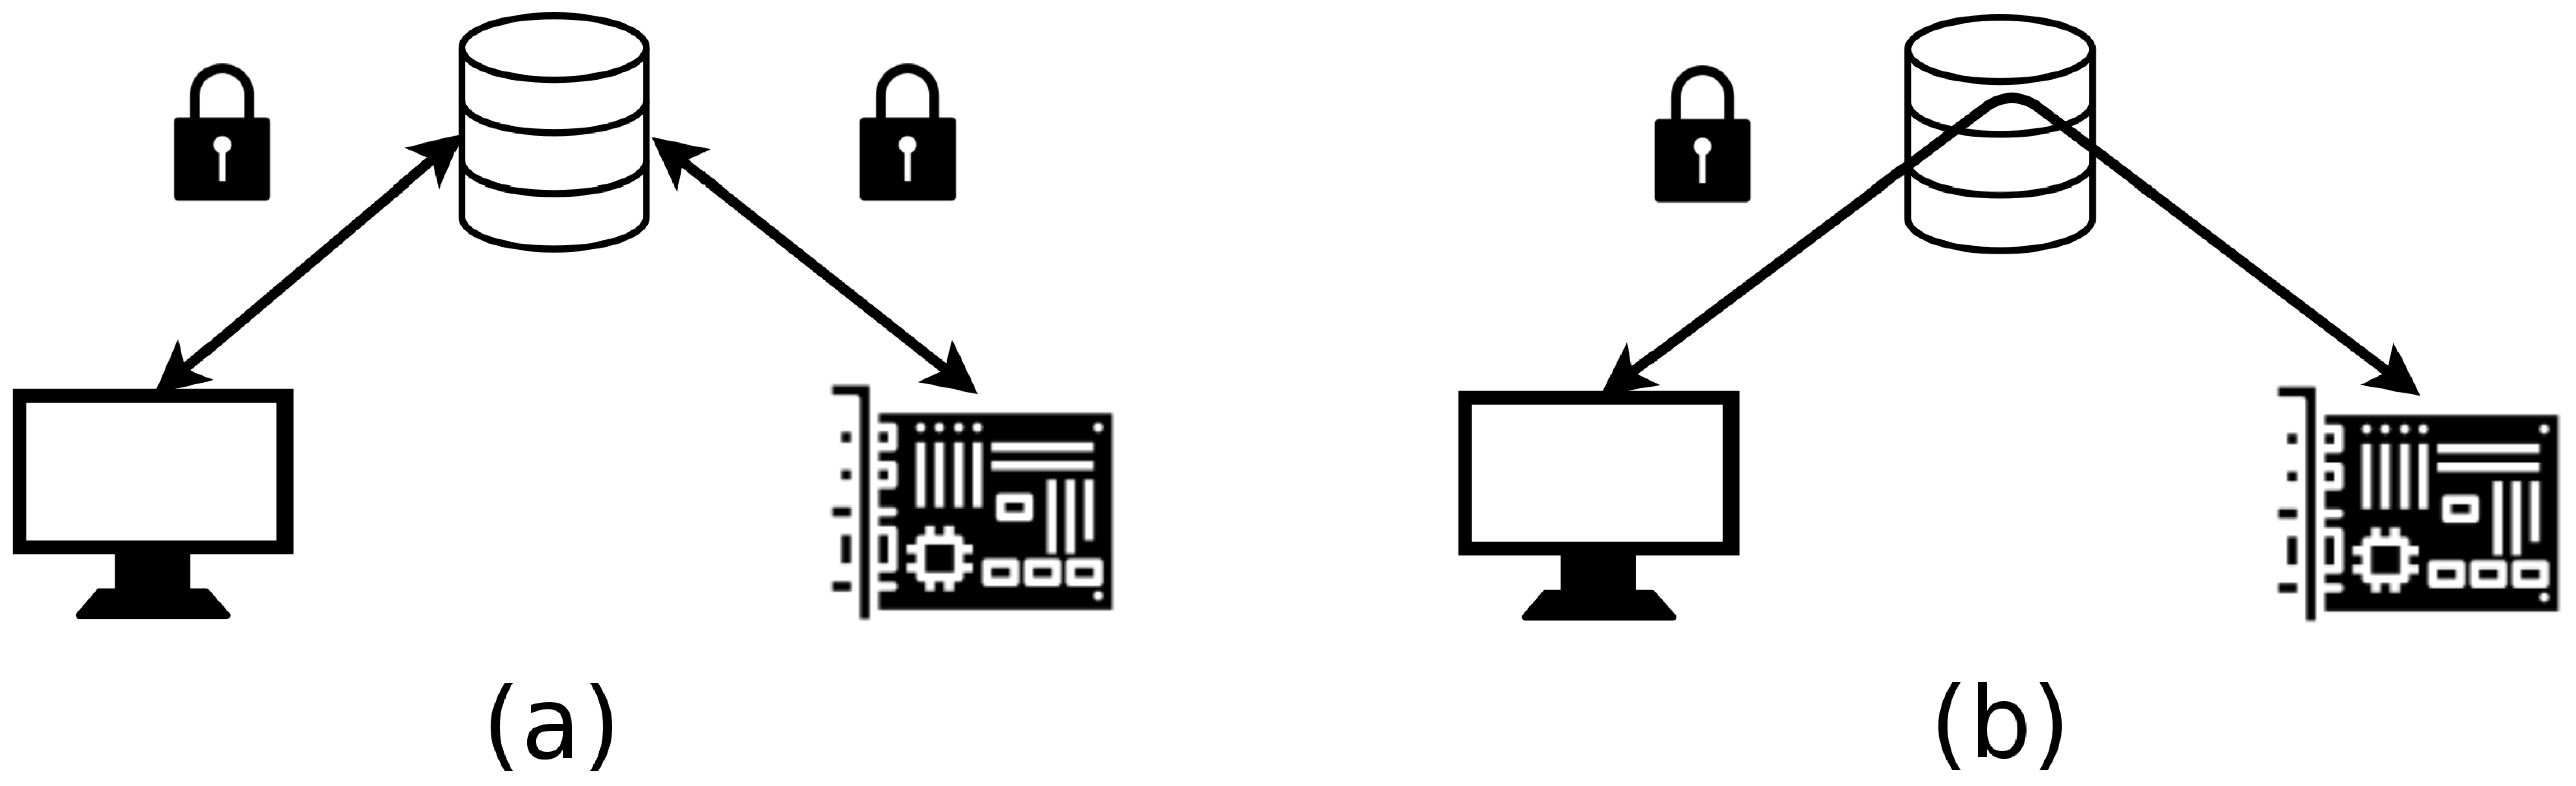
\includegraphics[width=0.8\textwidth]{papers/oscore/images/secure_comm}
\caption{Hop-by-hop vs. end-to-end security}
\label{fig:secure_comm}
\end{figure}

The original CoAP specification \cite{rfc7252} indicates DTLS \cite{rfc6347} as the only method to achieve secure communication for CoAP. This in turn means that, when a proxy is deployed between a client and server, message protection is enforced \emph{hop-by-hop} between client, proxies and server, as shown in Figure \ref{fig:secure_comm}(a). Thus, in the presence of an intermediary proxy, DTLS cannot provide \emph{end-to-end} secure communication between a client and server node. Instead, a first secure channel has to be established between the client and the proxy, and a second secure channel has to be established between the proxy and the server. This in turn results in the issues and limitations discussed in Section \ref{s:introduction}, i.e. the double security processing on the proxy as well as having to fully trust the proxy.

Figure \ref{fig:secure_comm}(b) shows the alternative \emph{end-to-end} security approach, where a client and a server rely on a two-way secure communication context. This approach essentially consists in tunneling channel security through the proxy, and hence successfully overcomes the two limitations discussed before. However, in order to be practically deployable and functional, a solution based on end-to-end security must not prevent proxies to correctly perform their intended functionalities, especially the caching of CoAP requests. Therefore it must be possible to \emph{selectively} protect different parts of a same CoAP message in different ways, i.e. some encrypted, others only integrity protected and finally some parts fully accessible by the proxy.

This flexibility can be achieved by using \emph{object security}, so that applications can choose which parts of an outgoing message have to be integrity-protected, encrypted, or both. Note that protecting only the CoAP payload is not sufficient against attacks such as changing the REST \emph{Code} field in the CoAP header, e.g. from \emph{GET} to \emph{DELETE}, which tricks the server into deleting a resource instead of just returning its value. 

The above motivates a need for lightweight end-to-end security with preserved proxying functionality, and has in turn led to the design of OSCORE, an application-layer protocol based on object security, which fulfills these requirements.


\section{Protocol description}
\label{sec:protocol}

%The code size of the cn-cbor library \cite{cite:cn-cbor} (constrained device
%CBOR) is roughly 1.4KB for an embedded ARM-Cortex-M3 platform.

\label{sec:oscoap}
This section describes Object Security for Constrained RESTful Environments (OSCORE). For the reader's convenience and due to space constraints, we only present the main features, while a complete description is available at \cite{cite:oscoap}.  OSCORE provides message confidentiality, integrity and reordering/replay protection, as well as a weak freshness protection through sequence numbers for CoAP messages. To this end, OSCORE transforms an \textit{unprotected CoAP message} into a \textit{protected CoAP message}. A protected CoAP message includes the newly defined \emph{OSCORE option} \cite{cite:oscoap}, which signals the usage of OSCORE to protect the message, as well as an encrypted COSE object \cite{rfc8152} in the CoAP payload. 

OSCORE is designed for providing end-to-end security between two CoAP endpoints, while preventing intermediaries to alter or access any message field that is not related to their intended operations. The security concerns not only the actual payload of the original CoAP message, but also all the fully protected CoAP options, the original request and response REST code, as well as parts of the URI to resources targeted in request messages (see Section \ref{ss:proxy_func}). 

To be able to use OSCORE, the following two criteria must be fulfilled. First, the two CoAP endpoints are required to support CBOR and COSE (see Section \ref{sec:cose}), as well as the specific \emph{HMAC-based Key Derivation Function} (HKDF) and \emph{Authenticated Encryption with Associated Data} (AEAD) algorithms they want to use for key derivation and authenticated encryption, respectively. This assumption is often already fulfilled in the vast majority of IoT applications using CoAP. Second, the two CoAP endpoints are required to have an OSCORE security context (see Section \ref{sec:con}), or the necessary information and keying material to derive it. While this has to happen in a secure and authenticated way, and some suitable approaches are proposed in \cite{cite:coseecdh}\cite{cite:oscoreprofile}, OSCORE is not tied to any particular approach for context establishment, and further details are out of the scope of this paper.

\subsection{The security context}
\label{sec:con}
OSCORE uses parameters and keying material included in an OSCORE \emph{security context}, and used to perform encryption and integrity protection operations. For this reason, every pair of communication endpoints, i.e. a CoAP client and a CoAP server, share the same security context.

The security context consists of three parts:  a \emph{Sender} part, a \emph{Recipient} part and a \emph{Common} part. The \emph{Sender} part is used to protect outgoing messages (i.e. requests on the client and responses on the server). The \emph{Recipient} part is used to verify incoming protected messages (i.e. requests on the server and responses on the client). Finally, the \emph{Common} part contains shared data. This division is illustrated in Figure \ref{fig:security_context}. An instance of a security context is present as a copy on the client and server, containing the same data values. However, as can be seen in Figure \ref{fig:security_context}, the sender and recipient parts are mirrored, so that the sender part of the server corresponds to the recipient part of the client, and vice versa.
\begin{figure}[ht]
    \centering
     \includegraphics[width=\textwidth]{papers/oscore/images/OSCORE_contexts.pdf}
    \caption{OSCORE Security Contexts for a Client and Server pair showing only the fields used during operation.}
    \label{fig:security_context}
\end{figure}{}

In more detail, the \emph{Common} part includes: i) an identifier of the AEAD algorithm used to encrypt and authenticate exchanged messages; ii) an identifier of the HMAC-based key derivation function used to derive keys and initialization vectors (IVs); iii) the \emph{Master Secret}, a random byte string used to derive keys and IVs; iv) the \emph{Master Salt}, an optional byte string used with the Master Secret to derive the keys and IVs; v) a Context ID, used to identify the Common Context and to derive keys and IVs; vi) a Common IV to generate AEAD nonces.

The \emph{Sender} part includes: i) a \emph{Sender ID}, a byte string identifying the \emph{Sender} part of the security context; ii) a \emph{Sender Key}, the symmetric key to protect outgoing messages; iii) a \emph{Sequence Number}, used for nonce generation to protect outgoing messages, and for replay protection of incoming messages (see Section \ref{sec:repl}).

The \emph{Recipient} part includes: i) a \emph{Recipient ID}, a byte string identifying the \emph{Recipient} part of the security context; ii) a \emph{Recipient Key}, the symmetric key to decrypt incoming messages; iii) a \emph{Replay Window} to verify freshness of incoming messages on the CoAP server (see Section \ref{sec:repl}).

The combination of Context ID, Sender ID, Master Secret and Master Salt must be unique for each communicating pair of Client and Server. This ensures unique keys and nonces for the AEAD. Further details on establishing Sender/Recipient IDs and the ensuring their uniqueness are out of the scope of OSCORE and of this paper.

\subsection{Protecting the CoAP message}
\label{ss:COSE_object}

Different parts in a CoAP message are protected in different ways. That is, \textit{Confidential data}, which should neither be read or altered by a proxy, are both encrypted and integrity protected. \textit{Static data}, which should be readable but not changed, are integrity protected but not encrypted. \textit{Dynamic data}, which a proxy should be able to modify, are not protected. Finally, there are also \textit{Mutually known data}, which the sender and receiver have agreed upon before exchanging messages. These data are part of the input to the integrity protection process, to ensure that the two communicating endpoints behave correctly and possibly detect anomalies. However, they are never sent as both parties already know them.

Figure \ref{fig:prot_struct} shows a comparison between an unprotected CoAP message and the resulting OSCORE-protected CoAP message. We can see that sensitive parts of a message are encrypted, e.g. some options and the payload, while others are left unencrypted, e.g. some options and some fields of the CoAP header. The encrypted content is placed into the payload of the protected message.

\begin{figure*}
\centering
   \begin{subfigure}[b]{\textwidth}
   \centering
     \begin{bytefield}[bitwidth=.9em]{32}
        %\bitheader{0-31} \\
         \bitbox{5}{Version} & \bitbox{4}{Type} & \bitbox{7}{Token Length} & \bitbox{8}{CoAP-Code} & \bitbox{8}{Message ID} \\
         \wordbox{1}{Token} \\
        \bitbox{9}{Option A} & \bitbox{6}{Option B} & \bitbox{6}{Option C} & \bitbox{11}{Option D} \\
        \bitbox{8}{Payload delimiter} & \bitbox{24}{CoAP-Payload}  \\
    \end{bytefield}
    \caption{CoAP message format.}
    \label{fig:coap-header}
   \end{subfigure}
  \newline
  \newline
    \begin{subfigure}[b]{\textwidth}
    \centering
    \begin{bytefield}[bitwidth=.9em]{32}
        %\bitheader{0-31} \\
         \bitbox{5}{Version} & \bitbox{4}{Type} & \bitbox{7}{Token Length} & \bitbox{8}{CoAP-Code} & \bitbox{8}{Message ID} \\
         \wordbox{1}{Token} \\
        %\bitbox{6}{Option B} & \bitbox{8}{11111111} & \bitbox[tlr]{24}{}  \\
        \bitbox{6}{Option B} & \bitbox{8}{OSCORE Option} & \bitbox{8}{Payload delimiter} & \bitbox[tlr]{10}{}  \\
        \wordbox[blr]{1}{Encrypted\{\footnotesize{Option A, Option C, Option D, CoAP-Code, CoAP-Payload}\} $+$ AEAD-tag} \\
    \end{bytefield}
    \caption{OSCORE message format.}
    \label{fig:oscore-header}
  \end{subfigure}
  \caption{Message layout for unprotected and protected CoAP messages.}
  \label{fig:prot_struct}
\end{figure*}

The actual protection process takes as input an unprotected CoAP message and produces a protected OSCORE message as follows.

\noindent
\textbf{1)} The confidential data are enclosed into a \textit{COSE object} \cite{rfc8152}. These include the REST code of the original CoAP message, a subset of the CoAP options, and the CoAP payload (if present). The CoAP options considered at this step are the ones not relevant for operations of intermediary (proxy) units.

\noindent
\textbf{2)} The static fields of the CoAP header and static proxy-readable CoAP options needs to be authenticated and integrity protected, but not to encrypted. This set of data composes the \emph{Additional Authenticated Data} (AAD).

\noindent
\textbf{3)} The COSE object is finalized, by encrypting and integrity protecting the data it encloses, while only integrity protecting the AAD. To this end, the Sender Key and the Sender Sequence Number from the Sender Context are used. The resulting \emph{ciphertext} and \emph{AEAD-tag} is included in the \emph{Message Content} field of the COSE Object.

\noindent
\textbf{4)} The COSE object is used as payload of the protected CoAP message, and any encrypted options are removed from the CoAP message. The original REST code is replaced with POST (2.04) for a CoAP request (response), or with FETCH (2.05) for a CoAP request (response) using the \emph{Observe} mechanism \cite{rfc7641}.

An analogous reverse process is performed upon receiving a protected message, together with anti-replay checks (see Section \ref{sec:repl}). To decrypt the protected message, the recipient CoAP endpoint uses the Recipient Key from its own Recipient Context associated to the message originator.




\subsection{Proxy functionalities and data protection}
\label{ss:proxy_func}
Building on the previous sections, we can now describe how OSCORE handles proxying of encrypted messages. OSCORE is designed to uniquely bind each request to the corresponding response, thus preventing proxies from serving cached responses to clients different from the one originating the request.

%OSCORE supports forward proxy functionalities, which affects the parts of CoAP messages accessed by forward proxies. That is, not all the data in the CoAP message can be encrypted, as some must remain readable to allow proxies to operate correctly. However, it is mostly possible to integrity protect such data.

As previously stated, OSCORE cannot encrypt entire CoAP messages. An example of static data in a CoAP message which can not be encrypted but should be integrity protected is the \emph{Version} field of the CoAP header. This field has to remain readable, so that the receiver endpoint knows how to process an incoming message, but should be integrity protected to prevent future version-based attacks.

The \emph{Token} field of the CoAP header also has to remain readable, as it is used for binding each request to the corresponding response. However, unlike the \emph{Version} field, the \emph{Token} field cannot be integrity protected, as it can be modified by proxies, when a message traverses the network.

\subsection{Replay protection}
\label{sec:repl}
OSCORE provides protection against replay and message reordering attacks. To this end, both the client and server store a sequence number and a replay window as part of the security context (see Section \ref{sec:con}) and including said sequence number in every outgoing request, before incrementing it by 1. Upon receiving a protected request, the server verifies that the conveyed sequence number was not received before. To correctly handle messages received out of order, OSCORE relies on a sliding window of sequence numbers, where the server accepts only messages with sequence number greater than the lower bound of the replay window. In such a case, the server updates its replay window accordingly. Otherwise, the server considers the message to be a retransmission and discards it.

\section{Evaluation of Payload and Network Overhead}
\label{s:payloadoverhead}
To aid reasoning and facilitate further discussion in the next sections, we have analyzed the payload overhead in bytes, as introduced by DTLS and OSCORE with respect to plain CoAP. To ensure a fair comparison, we have considered the same AEAD cipher for both DTLS and OSCORE, namely AES-128-CCM-8. Tables \ref{fig:overhead_dtls} and \ref{fig:overhead_oscore} show the overhead of the two different protocols. The entry "AEAD Tag" refers to the resulting Integrity Check Value produced by the AEAD cipher.

\begin{table*}[h]

\captionsetup[subtable]{position = below}
\captionsetup[table]{position=top}
\begin{subtable}{0.3\linewidth}
\centering
\begin{tabular}{l|l}
Type    & 1  \\
Version & 2  \\
Epoch           & 2  \\
Sequence Number & 6  \\
Length          & 2  \\
AEAD Tag        & 8  \\ \hline
Total overhead           & 21
\end{tabular}
\caption{Overhead of a DTLS-record layer message (bytes).}
\label{fig:overhead_dtls}
\end{subtable}%
\hspace*{2em}
\begin{subtable}{0.3\linewidth}
\centering
\begin{tabular}{l|l|l}
                     & Request & Response \\
OSCORE Option Byte   & 1    & 1\\
OSCORE Flag Byte     & 1    & -\\
Partial IV           & 0-5  & -\\
Kid                  & 0-7  & -\\
CoAP Code            & 1    & 1\\
Payload Marker       & 1    & 1\\
AEAD Tag             & 8    &  8\\ \hline
Total overhead       & 12-24 & 11
\end{tabular}
\caption{Overhead of an OSCORE message (bytes).}
\label{fig:overhead_oscore}

\end{subtable}
\caption{Payload overhead for DTLS 1.2 and OSCORE.}
\end{table*}

As we can see in Table \ref{fig:overhead_dtls}, DTLS displays a fixed overhead of $21$ bytes, which is equal for both requests and responses. This results in a total overhead of $42$ bytes for a full message exchange. Note that, as defined in the DTLS profile for IoT in \cite{rfc7925} (Appendix B), devices using DTLS are expected to additionally include an $8$-byte explicit nonce to the DTLS header. This would result in an overhead of $29$ bytes per message, i.e. of $58$ bytes for each two-way message exchange.

In OSCORE, the overhead can vary, due to the following reasons. First, the "Partial IV" field in the OSCORE option includes the message sequence number, whose value is incremented and size grows over time as Requests are transmitted, up to a maximum size of $5$ bytes. Second, the "Kid" field (Key Id) in the OSCORE option is immutably set by the user during early configuration, with possible sizes ranging between $0$ (empty Key Id) and $7$ bytes. 

With reference to Table \ref{fig:overhead_oscore}, we can see that, as long as the Key Id is chosen to have a length of maximum $4$ bytes, OSCORE will display the same or lower overhead for all Requests. Note that a Key Id of maximum $2$ bytes is expected to be the practical choice for most applications using OSCORE. Furthermore, OSCORE Responses omit a number of implicit fields in the OSCORE option, and thus showing a smaller fixed overhead of $11$ bytes. Note that, unlike DTLS, OSCORE has a (much) smaller overhead for responses than requests. Assuming a high-value Partial IV of $5$ bytes and a Key Id of $2$ bytes, this would result in an overhead of $19$ bytes per request message and of $11$ bytes per response message, i.e. of $30$ bytes for a two-way message exchange.

Also, an application relying on IEEE 802.15.4 typically displays an effective data rate (i.e. excluding headers, CRCs and control packets) of about $8.4$ kbit/s (out of $250$ kbit/s). However, as shown by Latr\'{e} \emph{et al.}, IEEE 802.15.4 networks can actually achieve a throughput of about $140$ kbit/s, even if acknowledgement frames are transmitted \cite{latre:2005}. Using these numbers together with the energy consumption numbers stated in the CC2538 datasheet\footnote{\url{http://www.ti.com/lit/ds/symlink/cc2538.pdf}}, we get the numbers shown in Table \ref{tab:overhead}.
\begin{table}[h]
\center

\begin{tabular}{l|ll|ll}
         & \multicolumn{2}{l}{Time (ms)} & \multicolumn{2}{l}{Energy ($\mu J$)} \\ 
         & DTLS         & OSCORE         & DTLS                   & OSCORE                  \\ \hline
Request  & 1.2          & 1.086          & 95.04                  & 71.676                  \\
Response & 1.2          & 0.628          & 79.2                   & 49.738                  \\
Exchange & 2.4          & 1.714          & 174.24                 & 121.414                

\end{tabular}
\caption{Overhead in transmission time and energy consumption for a cc2538 server receiving and sending DTLS and OSCORE messages.}
\label{tab:overhead}
\end{table}

\section{Experimental Evaluation Method}
\label{sec:measure}

To evaluate the feasibility and convenience of OSCORE, we developed a prototype implementation for resource-constrained CoAP servers. This section presents the conducted experiments which evaluates the performance of OSCORE. We chose to evaluate OSCORE against both plain CoAP and CoAP secured with DTLS since CoAP recommends DTLS as a security mechanism. The plain CoAP scenario, namely "COAP", acts as a baseline comparison for the DTLS-based scenario, namely "COAPS", and for the OSCORE-based scenario, namely "OSCORE". We show that, even with no particular optimizations, OSCORE displays an affordable overhead, and outperforms DTLS in terms of resource utilization and energy consumption on the server side, as well as responsiveness perceived on the client side.

%TODO, perhaps we should change the picture to include the proxy.
% M.T. Agree. Also, "Radio" can be renamed to "IEEE 802.15.4 link"
\begin{figure}[!htbp]
\centering
%images are free to use without attribution (https://iconmonstr.com/cpu-2-eps/)
\begin{tikzpicture}[scale=1,every node/.style={outer sep=.2cm}]
\node (client) at (0,0) {\includegraphics[height=1cm]{papers/oscore/images/iconmonstr-laptop-6.pdf}};
\node[right = 1.7cm of client] (proxy)  {\includegraphics[height=1cm]{papers/oscore/images/iconmonstr-laptop-6.pdf}};
\node[right = 1.7cm of proxy] (router) {\includegraphics[height=.8cm]{papers/oscore/images/iconmonstr-radio-tower-1.pdf}};
\node[right = 1.7cm of router] (server) {\includegraphics[height=1cm]{papers/oscore/images/iconmonstr-cpu-2.pdf}};


\node[above = -0.3cm of client] (client-h) {\scriptsize Client};
\node[above = -0.3cm of proxy] (proxy-h) {\scriptsize Proxy};
\node[above = -0.2cm of router] (router-h) {\scriptsize Border Router};
\node[above = -0.3cm of server] (server-h) {\scriptsize Server};

\draw[<->]([xshift=0cm]client.east) -- ([xshift=-0cm]proxy.west) node [midway, above] (usb) {\tiny IP};
\draw[<->]([xshift=0cm]proxy.east) -- ([xshift=-0cm]router.west) node [midway, above] (usb) { \tiny USB};
\draw[<->]([xshift=0cm]router.east) -- ([xshift=-0cm]server.west) node [midway, above] (radio) { \tiny IEEE 802.15.4};

\end{tikzpicture}
\caption[Test set-up]{Experimental test scenario.}
\label{fig:setup}
\end{figure}

For our experiments, we considered the test scenario in Figure \ref{fig:setup}, which consists of a CoAP client, a CoAP proxy and a CoAP server. The client (C) and the proxy (P) were implemented using an extended version of the Java library Californium/Scandium \footnote{\url{http://www.eclipse.org/californium}}, which provides both CoAP and DTLS. The client and the proxy ran as two distinct processes on a same commodity PC. To enable communication between P and the server (S), we relied on a dedicated border router (BR) device. In particular, both BR and S were resource-constrained Zolertia Firefly boards \footnote{\url{https://zolertia.io/product/firefly}}, and ran the Contiki-NG OS \footnote{\url{https://github.com/contiki-ng/contiki-ng/wiki}} together with an extended version of the Erbium library providing the communication stack. The Firefly boards are based on the CC2538 chipset and equipped with 512 KB of ROM, 32 KB of RAM, a 32 MHz ARM Cortex-M3 CPU, and an IEEE 802.15.4 \cite{IEEEStd802.15.4} radio interface.

We considered and compared three different test cases: "COAP", "COAPS" and "OSCORE". In all three test cases, P acts as CoAP proxy and relays CoAP requests from C to S, as well as corresponding CoAP responses from S to C. More specifically, the three test cases were defined as follows.

\noindent
$\bullet$ \textbf{"COAP"}. The "COAP" test case considered plain CoAP communication, with no security provided.

\noindent
$\bullet$ \textbf{"COAPS"}. The "COAPS" test case considered CoAP communication with the addition of DTLS 1.2, providing hop-by-hop secure communication. DTLS was configured with a first secure channel between C and P, and a second secure channel between P and S. Both DTLS channels used the DTLS ciphersuite TLS\_PSK\_WITH\_AES\_128\_CCM\_8 \cite{rfc6655}.

\noindent
$\bullet$ \textbf{"OSCORE"}. The "OSCORE" test case considered CoAP communication with the addition of OSCORE, providing end-to-end secure communication between C and S, as described in Section \ref{sec:protocol}.

Note that neither "COAPS" nor "OSCORE" relied on hardware acceleration for cryptographic operations, and that "COAP" does not make use of cryptography.

In all three test cases, the client sent POST requests addressed to a dedicated target resource at the server S. Also, S was configured to reply to each such request by sending a response with the same payload size. The client was pre-configured in order to skip the resource discovery process.

In the considered setup, the server did not rely on the Radio Duty Cycling mechanism provided by Contiki for switching off the node's radio interface if not in use \footnote{\url{https://github.com/contiki-os/contiki/wiki/Radio-duty-cycling}}. In the "COAPS" and "OSCORE" test cases, the involved parties had already established a security association which enabled a secure message exchange. That is, the completion of the DTLS handshake, as well as the establishment of OSCORE security contexts, were out of scope for this paper and our performance evaluation, which focused on the (secure) exchange of messages.

For each test case, we performed separate experiments. During a given experiment, the payload size of every CoAP message was either $1$, $16$, $32$, $48$, $64$, $80$, $96$, $112$ or $128$ bytes. For each listed payload size, we performed $500$ message exchanges between the client and the server, through the proxy. In all the test cases, we performed the following measurements: i) Responsiveness as experienced by C for a message exchange with S; ii) CPU usage by the server; iii) Memory usage by the server, i.e. RAM and ROM; iv) Radio usage by the server; and v) Energy usage by the server. In particular, we performed the measurements as follows.

\noindent
\textbf{Responsiveness}. We evaluated the Round Trip Time (RTT), as experienced by the client when performing a full Request-Response exchange. The statistical significance of these results were verified with the method of paired t-tests.

\noindent
\textbf{CPU usage}. We measured the execution time needed to process both incoming messages from a client and  outgoing response messages. For the "COAPS" and "OSCORE" test cases, this includes decryption and integrity verification of incoming messages, as well as encryption of outgoing messages. Paired t-tests were used for verification of statistical significance.

\noindent
\textbf{Memory usage}. The static memory utilization was determined by using the GNU utility \emph{size}. Since Contiki-NG does not use dynamic memory allocation on the heap, dynamic memory utilization is limited to the stack. Hence, in our experiments, we used the \textit{stack painting} painting technique, where a known value is written to all addresses of the stack part of the memory. After the experiments, the number of bytes that had been overwritten by the program execution were counted.

\noindent
\textbf{Radio usage}. We have measured the time needed by the server to receive and transmit messages using \emph{Energest}, a Contiki-NG utility for monitoring system utilization. Energest makes it possible to measure the time intervals where the CPU has been active, or where the radio interface has been active either in reception mode (RX) or transmission mode (TX). Furthermore, Energest has been proven to enable an accurate estimation of energy consumption, while increasing the computing time only of the $0.7\%$ \cite{energest}.

\noindent
\textbf{Energy usage}. We measured the energy consumed at the server, both by the CPU, and by the radio interface in transmission and reception mode. Each measurement was computed as the product between the overall related time collected by Energest, and the power consumption of the related hardware component as documented in the respective manuals\footnote{\url{https://zolertia.io/product/firefly}}\footnote{\url{http://www.ti.com/lit/ds/symlink/cc2538.pdf}}.

\section{Results and Discussion}
\label{sec:results}

This section presents and discusses the results of our experiments, with reference to the test cases and scenario described in Section \ref{sec:measure}. The data presented here represent the average for a single message from a sample set of $500$ messages.

\subsection{Responsiveness}
The top graph in Figure \ref{fig:rtt} shows the average RTT experienced by the client for different payload sizes, with the different curves showing the three different test cases. The bottom graph shows the calculated difference in mean response time between OSCORE and COAPS, with error-bars showing the standard deviation.

\begin{figure}[h]
\centering
\includegraphics[width=0.8\textwidth]{papers/oscore/images/rtt.png}
\caption[RTT measurements]{Measurement of responsiveness comparing RTT between COAP, COAPS and OSCORE. }
\label{fig:rtt}
\end{figure}

Table \ref{tab:tstat} shows the statistical significance (t-statistics and p-values) for the values in the bottom graph in Figure \ref{fig:rtt}. For each payload size, the statistics are derived using paired t-tests, comparing response time sample populations.

\begin{table}[h]
\centering
\caption {Statistical significance for RTT, (t-statistics and p-values)} \label{tab:title} 
\small\addtolength{\tabcolsep}{-2pt}
\begin{tabular}{c|c|c|c|c|c|c|c|c|c}
Payload \\ (Bytes)  & 1    & 16   & 32   & 48   & 64   & 80   & 96   & 112  & 128  \\ \hline
                  t & 7.8  & 3.2  & 14.5 & 12.2 & 1.0  & 3.0  & 1.7  & 13.8 & 1.9  \\ 
                  p & 0.0 & 0.0 & 0.0 & 0.0    & 0.30 & 0.0 & 0.09 & 0.0 & 0.06
\end{tabular}
\label{tab:tstat}
\end{table}

As it can be seen in Figure \ref{fig:rtt}, there is a notable difference in the mean response time between the protocols, with OSCORE being more efficient than COAPS for all payload sizes. The statistical significance of the difference, see Table \ref{tab:tstat}, is strong for most packet sizes, achieving a 99\% confidence interval. However, for 64, 96 and 128 bytes payload, statistical significance is not achieved. This is likely due to a large variance in transfer time on the IEEE 802.15.4 network. Overall, the lines in the top graph of Figure \ref{fig:rtt} resemble a staircase. Further investigation showed that this is due to package fragmentation.

\begin{figure}
\centering
\includegraphics[width=1.0\textwidth]{papers/oscore/images/frags.png}
\caption[Fragmentation measurements]{number of packages needed to transport a single message. }
\label{fig:frag}
\end{figure}

Figure \ref{fig:frag} shows the number of packages needed to transport one message for the different protocols and payloads. We can see that the biggest possible payload that can be carried in a single frame has a different size in the three scenarios, with COAP being able to fit the most data into a single frame and COAPS the least. This is because the total header sizes for the used protocols vary between the COAP, OSCORE and COAPS scenarios, i.e. $76$, $90$ and $105$ bytes, respectively. The Maximum Transmission Unit for a IEEE 802.15.4 network is 127 bytes.

\subsection{CPU usage}
Figure \ref{fig:parse} and Figure \ref{fig:serialize} show the CPU time for processing incoming and outgoing COAP, COAPS and OSCORE messages. The left graphs show the total CPU time for the different protocols, including cryptographic operations. The right graphs show the CPU time excluding cryptographic operations.
\begin{figure}[h]
\begin{subfigure}{1.0\textwidth}
\centering
\includegraphics[width=1.0\textwidth]{papers/oscore/images/proc.png}
\caption[Processing measurements]{Measurement of CPU time when processing incoming messages with COAP, COAPS and OSCORE. }
\label{fig:parse}
\end{subfigure}

\begin{subfigure}[h]{1.0\textwidth}
\centering
\includegraphics[width=1.0\textwidth]{papers/oscore/images/serialize.png}
\caption[Processing measurements]{Measurement of CPU time when processing outgoing messages with COAP, COAPS and OSCORE. }
\label{fig:serialize}
\end{subfigure}
\end{figure}

In particular, Figure \ref{fig:parse} shows the CPU-time for processing incoming messages. The left graph shows the total CPU-time for processing incoming messages with COAPS, OSCORE and COAP. The graph shows that OSCORE is faster than COAPS when processing incoming messages, for all message sizes. In the right graph of Figure \ref{fig:parse}, we show the CPU-time for processing incoming messages excluding the CPU-time spent for decryption. Here we see that OSCORE takes longer time than COAPS for all message sizes.

Similarly, Figure \ref{fig:serialize} shows the CPU-time for processing outgoing messages. The left graph shows the total CPU-time for processing outgoing messages with COAPS, OSCORE and COAP. Where cryptographic operations are taken into account, OSCORE is faster than COAPS when processing outgoing messages, for all messages sizes. In the right graph of Figure \ref{fig:serialize}, we show the CPU-time for processing outgoing messages excluding the CPU-time spent for encryption. Again, here we see that OSCORE takes longer time than COAPS for all message sizes. 

The observed difference between the right and left side of the graphs is due to the following reasons. Other than the actual encryption/decryption processing of messages, OSCORE is slower than DTLS due to: i) a more complex handling of OSCORE security contexts (i.e. retrieval and update), compared to the handling of DTLS sessions; ii) a more complex preparation of a protected OSCORE message from an original CoAP message and vice versa (see Section \ref{sec:protocol}), compared to the preparation of a protected DTLS record from an original CoAP message and vice versa. However, when also cryptographic operations are taken into account, OSCORE outperforms DTLS as more efficient in protecting/unprotecting handled messages. Ultimately, OSCORE achieves this result especially by leveraging a more efficient implementation of the AES-CCM algorithm.

The results in both Figure \ref{fig:parse} and Figure \ref{fig:serialize} are verified for statistical significance with 99\% confidence interval using a paired t-test. The results of these experiments show that the CPU performance for both protocols hinges on a fast cipher implementation. In these experiments we used software implementations of AES128-CCM. Hardware acceleration of the encryption will increase the performance of both OSCORE and COAPS.

\subsection{Memory usage}
Figure \ref{fig:memory} shows the memory usage results. In particular, the left bar chart shows the RAM usage, including the maximum stack usage, while the right bar chart shows the ROM usage. In order to be independent from the particular used cryptographic primitives, e.g. cipher and hash functions, the shown memory results do not include memory usage due to such primitives. Furthermore, since the DTLS Handshake protocol is not comparable against anything analogous in OSCORE, the memory usage due to the DTLS Handshake is also excluded from the shown results. Nevertheless, for the sake of information completeness, the right bar chart highlights the memory utilization due to such contributions with faded color areas at the top of the bars.

\begin{figure}[h]
\centering
\includegraphics[width=0.8\textwidth]{papers/oscore/images/memory.png}
\caption[Memory utilization]{Memory utilization. The lighter parts in the ROM usage graph on the right indicates the memory used for the DTLS Handshake (in the "COAPS" test case) and for cryptographic primitives (in the "COAPS" and "OSCORE" test cases).}
\label{fig:memory}
\end{figure}

We can see that OSCORE uses less RAM and ROM than DTLS. Furthermore, OSCORE only uses $2\%$ more RAM than COAP, while COAPS uses $17\%$ more RAM than COAP. When comparing the ROM usage excluding cryptographic primitives, OSCORE uses $12\%$ more ROM than COAP, while COAPS uses $27\%$ more ROM than COAP when excluding the DTLS Handshake protocol and cryptographic primitives.

\subsection{Radio usage}
Figure \ref{fig:energest} shows the radio utilization rates for the tested protocols. The left graph shows the percentage of time spent in transmit mode while the right graph shows the percentage of time spent in listening mode. 

\begin{figure}[h]
\centering
\includegraphics[width=0.9\textwidth]{papers/oscore/images/energest-radio.png}
\caption[Radio measurements]{Measurements of radio time occupancy for transmit and receive for the three protocols.}
\label{fig:energest}
\end{figure}

Compared to COAPS, OSCORE displays less radio usage when transmitting messages for most packet sizes. The time in listening mode is also smaller for OSCORE for most payload sizes. We conclude that OSCORE requires less network resources compared to COAPS.

These results were acquired using Energest, which uses timers to measure the time the radio has spent in either transmit-mode or receive-mode. Note that switching one timer off and the other on, e.g. going from transmit-mode to receive-mode cannot be done instantly. Therefore, the sum of the time in transmit-mode and the time in receive-mode does not always add up to the total elapsed time. However, the difference between these times and the error percentage is negligible.

\subsection{Energy usage}
We used Energest to measure the energy used for CPU, radio transmission and radio receiving by the different protocols for a message transaction. These results, along with a summation of total energy usage, can be seen in Figure \ref{fig:energy}.

\begin{figure}[h]
\centering
\includegraphics[width=0.8\textwidth]{papers/oscore/images/energest-energy.png}
\caption[Energy Consumption per exchange]{Energy consumption per message exchange. Note that scales are different for the y-axes.}
\label{fig:energy}
\end{figure}

We can see that the impact of the CPU power consumption is larger than the impact of the radio power consumption. A contributor to this is the fact that these CPU measurements include power consumed when the CPU idles in between messages (which are sent at a rate of 10 messages per second). This factor can be reduced by letting the CPU sleep instead of idling in between messages.

Most significant, we can see that OSCORE uses less energy in total compared to COAPS for all payload sizes. OSCORE has a per-exchange energy consumption about 8-28\% higher than COAP. This shows that OSCORE is more energy efficient than COAPS, which has an energy consumption about 17-59\% higher than COAP.

\section{Conclusion}
\label{sec:conclude}
We have presented OSCORE, a method for securing CoAP messages at the application layer based on object security. Unlike channel security approaches such as the DTLS protocol, OSCORE always ensures end-to-end security between client and server, even in the presence of intermediary (untrusted) proxies, with additional benefits in terms of privacy. OSCORE has been recently standardized as a security protocol at the Internet Engineering Task Force (IETF) \cite{cite:oscoap}. We have evaluated our implementation of OSCORE for the Contiki OS against DTLS on the SmartRF resource-constrained platform. Experimental results show that OSCORE outperforms DTLS in important metrics, namely radio transmission overhead, round trip time as experienced by CoAP clients, and memory usage as well as energy efficiency for constrained servers. Future work will focus on using OSCORE to secure multicast CoAP messages in use cases relying on group communication.

\section*{Acknowledgements}
The authors sincerely thank the anonymous referees and the associate editor for their insightful comments and suggestions. This work received funding from the European Union's Seventh Framework Programme for research, technological development and demonstration under grant agreement no. 607109. This work was also supported by the EIT-Digital High Impact Initiative ACTIVE; VINNOVA for the Celtic-Plus project CyberWI and the Celtic-Next project CRITISEC; SSF Grant RIT17-0032 and the Wallenberg AI, Autonomous Systems and Software Program (WASP) funded by the Knut and Alice Wallenberg Foundation. The authors thank Rikard H\"{o}glund and Jiye Park for their help and comments.


{\raggedright
        \printbibliography[segment=\therefsegment,heading=subbibliography]
}

